\begin{frame}
    \frametitle{Наборы данных для исследования}
    Для исследования качества решений и временной сложности алгоритма были созданы следующие наборы данных:
    \begin{enumerate}
        \item Набор данных с известным оптимумом.
        % \begin{itemize}
        %     \item 2000; 5000; 10000; 20000; 30000; 40000; 50000; 75000; 100000 работ
        % \end{itemize}
        \item Набор данных, основанных на слоистых данных.
        % \begin{itemize}
        %     \item 
        % \end{itemize}
        \item Набор данных для построения расписания на неоднородных процессорах.
        % \begin{itemize}
        %     \item 
        % \end{itemize}
    \end{enumerate}
\end{frame}

\begin{frame}
    \frametitle{Точность полученного расписания. CR}
    \begin{figure}
        \begin{subfigure}{0.49\textwidth}
            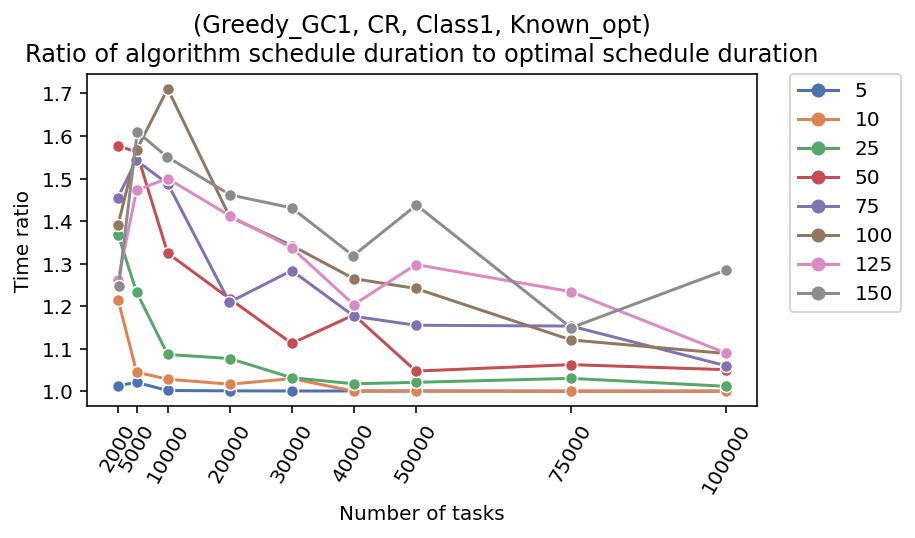
\includegraphics[width=\textwidth]{imgs/ideal_1/CR/gr_amalgamated.png}
            \caption{Жадный алгоритм с выбором по числу потомков}
        \end{subfigure}
        \begin{subfigure}{0.49\textwidth}
            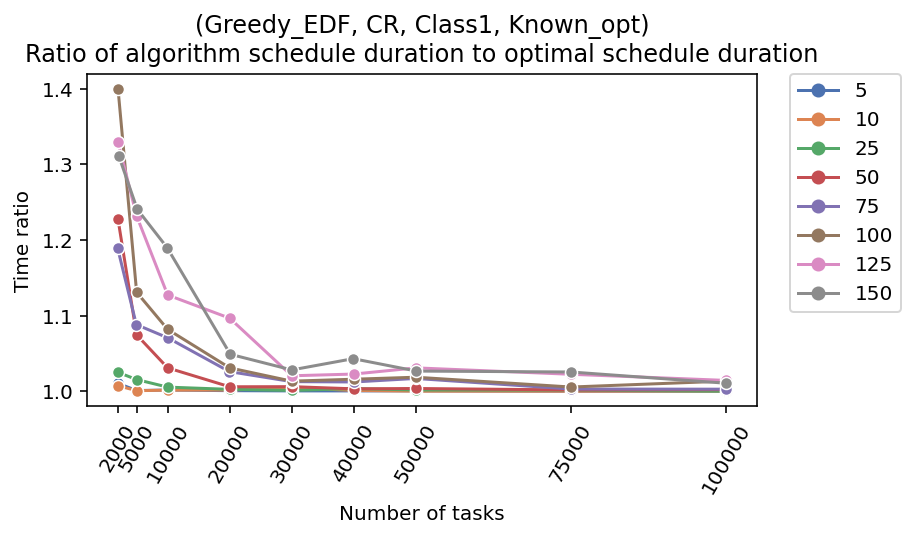
\includegraphics[width=\textwidth]{imgs/ideal_1/CR_EDF/gr_amalgamated.png}
            \caption{Жадный алгоритм с фиктивными директивными сроками}
        \end{subfigure}
        \caption{Качество решений алгоритмов на данных с известным оптимумом,\\ постановка с дополнительным ограничением на межпроцессорные передачи}
    \end{figure}
\end{frame}

\begin{frame}
    \frametitle{Точность полученного расписания. NO}
    \begin{figure}
        \begin{subfigure}{0.49\textwidth}
            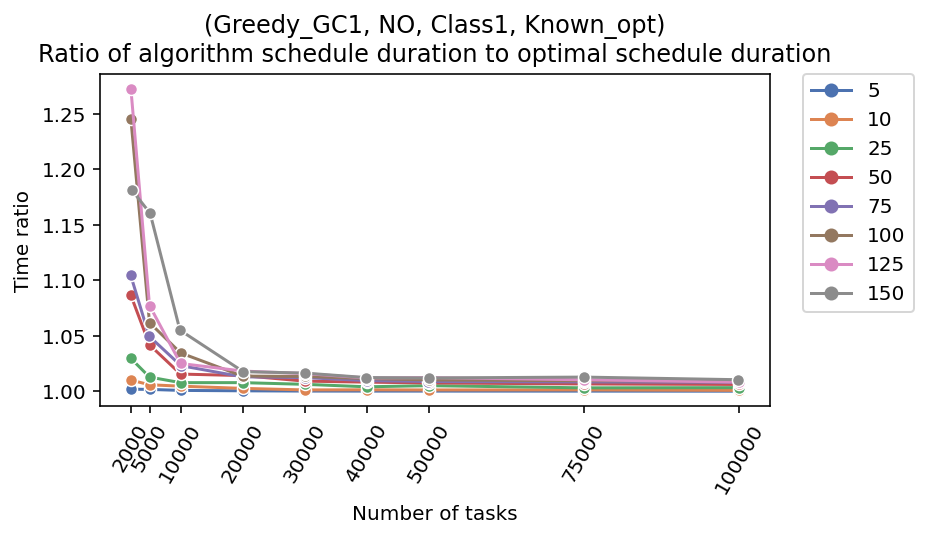
\includegraphics[width=\textwidth]{imgs/ideal_1/NO/gr_amalgamated.png}
            \caption{Жадный алгоритм с выбором по числу потомков}
        \end{subfigure}
        \begin{subfigure}{0.49\textwidth}
            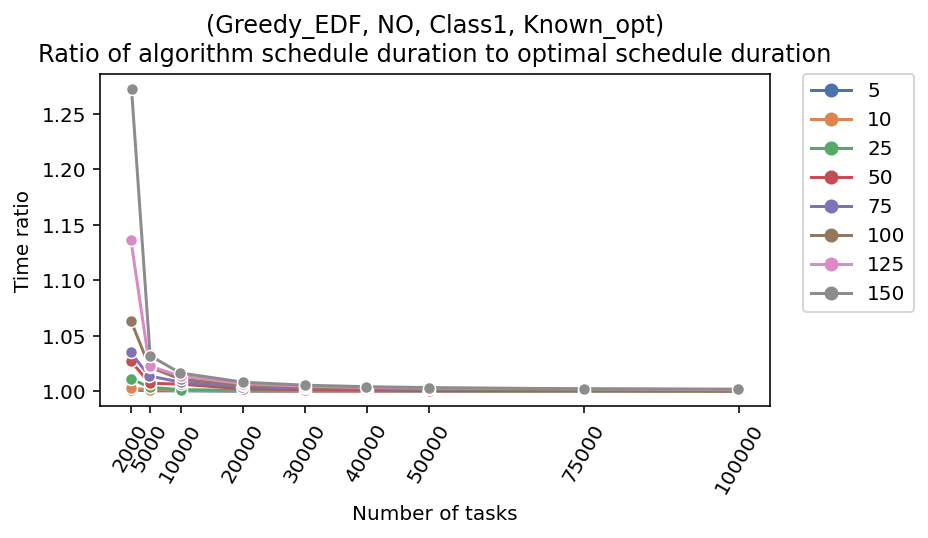
\includegraphics[width=\textwidth]{imgs/ideal_1/NO_EDF/gr_amalgamated.png}
            \caption{Жадный алгоритм с фиктивными директивными сроками}
        \end{subfigure}
        \caption{Качество решений алгоритмов на данных с известным оптимумом,\\ постановка без дополнительных ограничений}
    \end{figure}
\end{frame}

\begin{frame}
    \frametitle{Программная реализация алгоритма}
    \begin{columns}
        \begin{column}{0.5\textwidth}
            \begin{figure}
                \centering
                \begin{tikzpicture}
                    \tiny
                    \begin{class}{ScheduleData}{0, 0}
                        \attribute{+ tran\_times : boost::numeric::ublas::matrix}
                        \attribute{+ task\_times : boost::numeric::ublas::matrix}
                        \attribute{- graph : Graph}
                    \end{class}
            
                    \begin{class}{TimeDiagram}{0, -2.2}
                        \attribute{+ proc\_array : std::vector<std::list<PlacedTask>>}
                        \operation{+ extract\_data(conf : greedy\_config) : Output\_data}
                    \end{class}
            
                    \begin{class}{OutputData}{0, -4.2}
                        \attribute{+ CR : double}
                        \attribute{+ criteria : opts::greedy\_config::extra\_criteria}
                        \attribute{+ nodes : unsigned int}
                        \attribute{+ time : unsigned long}
                        \attribute{+ proc\_array : std::vector<std::list<PlacedTask>>}
                    \end{class}
            
                    \begin{class}[text width=2.7cm]{GreedyConfig}{5, 0}
                        \attribute{+ criteria : extra\_criteria}
                        \attribute{+ CR\_bound : double}
                        \attribute{+ \_class : input\_class}
                    \end{class}
                    
                    \begin{class}[text width=3cm]{PlacedTask}{5, -5}
                        \attribute{+ task\_no : unsigned int}
                        \attribute{+ start : unsigned int}
                        \attribute{+ finish : unsigned int}
                    \end{class}
            
                    \composition{TimeDiagram}{sched}{}{ScheduleData}
                    \composition{ScheduleData}{conf}{}{GreedyConfig}
                \end{tikzpicture}
                % \caption{UML-диаграмма реализации}
                \label{fig:UML}
            \end{figure}
        \end{column}
        \begin{column}{0.5\textwidth}
            Программная реализация была выполнена на языке \texttt{C++}, с использованием библиотек \texttt{boost}, \texttt{METIS}, \texttt{json} и \texttt{toml}. Реализация занимает 1689 строк.
        \end{column}
    \end{columns}
\end{frame}

